\section{DNA-like oxidation of MoRe thin films}
\label{sec:more}

During his times as postdoc at TU Delft, my supervisor Gary Steele found that the superconducting alloy molybdenum-rhenium was the only suitable superconductor to sustain the growth conditions of carbon nanotubes.
Moreover, the work function of MoRe matches that of graphene quite close, which was why its use was further pushed in the field of hybrid carbon-superconductor devices.
However, it was often overlooked that devices made from MoRe began exhibiting peculiar "spots" visible under an optical microscope after a few days.

We found that there were small "crystallites" growing on the surface of sputtered MoRe films, regardless of wafer substrate and film thickness.
Growth of these structures seems to be forming by seed-growth of small islands less than \SI{1x1}{\micro\meter} in size (cf. Figs.~\ref{fig:MoreDNA}C,D) which would then diffuse on the surface and cluster together in DNA-like strands (cf. Fig.~\ref{fig:MoreDNA}B).
This growth mechanism covers the entire film surface with small islands, lumping together into bigger structures, as depicted in Fig.~\ref{fig:MoreDNA}A.
Remarkably, some of the largest crystals grew even higher in the third dimension than the original MoRe film thickness.

Analzying the atomic composition of these crystallites using EDX peak intensity lead us to believe that the they are mainly composed of rhenium oxide, judging from the reduced molybdenum EDX peak intensity compared to the one of rhenium at these spots, cf. Fig~\ref{fig:moreedx}.
The signal originating from the silicon peak (c) is expected to be weaker at the crystal location since due to less X-ray radiation can reach the detector because of the increase in thickness.
In contrast to the reduced silicon and molybdenum peaks, the oxygen and rhenium signals are stronger at the crystal location, strongly hinting at some kind of rhenium oxide.

Further, quantitative compositional analysis could not be performed because the oxygen signal is very close to the zero loss peak and the rhenium and molybdenum content of the surface layer would have some contribution of the bulk below.
Our observation contrasts the one made on thin and bulk MoRe structures in literature, where \ce{MoO3} and \ce{MoO2} were found to be the dominant oxide~\cite{seleznevDepositionCharacterizationFewnanometersthick2008b,gotzCosputteredMoReThin2016}.
To the best of our knowledge, there is however no literature on the observed ReO crystallites.

While the superconducting critical temperature of large structures of this film seemed to be unaffected by the growth, these structures can severely degrade the high-frequency response of superconducting circuits such as resonators or qubits, as dielectric losses can be one of the main reasons for qubit decoherence~\cite{lisenfeldElectricFieldSpectroscopy2019}.
Moreover, since the crystallites physically move about on the film surface, they might interfere with any patterned structures, leading to unintended defects in or even damage the electrical wiring.
We found that a \SI{60}{\second} dip of MoRe films in strong oxidizing agents, such as MF321 or BOE, was enough to wash off these crystallites as longs as they were still in the seed phase, and the density of big clusters was low.
This corresponds to a storage time below three days in ambient conditions.
Crystal seeding sets in almost immediately and is clearly visible under an optical microscope at 5x magnification after one day. 
The crystal growth can be slowed down significantly, but not completely suppressed, if films are stored in dry boxes with constant nitrogen flow.
We estimate that one day in ambient conditions has the same effect as two weeks in nitrogen atmosphere.

Since the devices studied in this thesis did not require MoRe per se, we chose to abandon this superconducting alloy after thorough investigation, and switched to NbTiN or aluminum, depending on the specific circuit requirements.

\begin{figure}
	\centering
	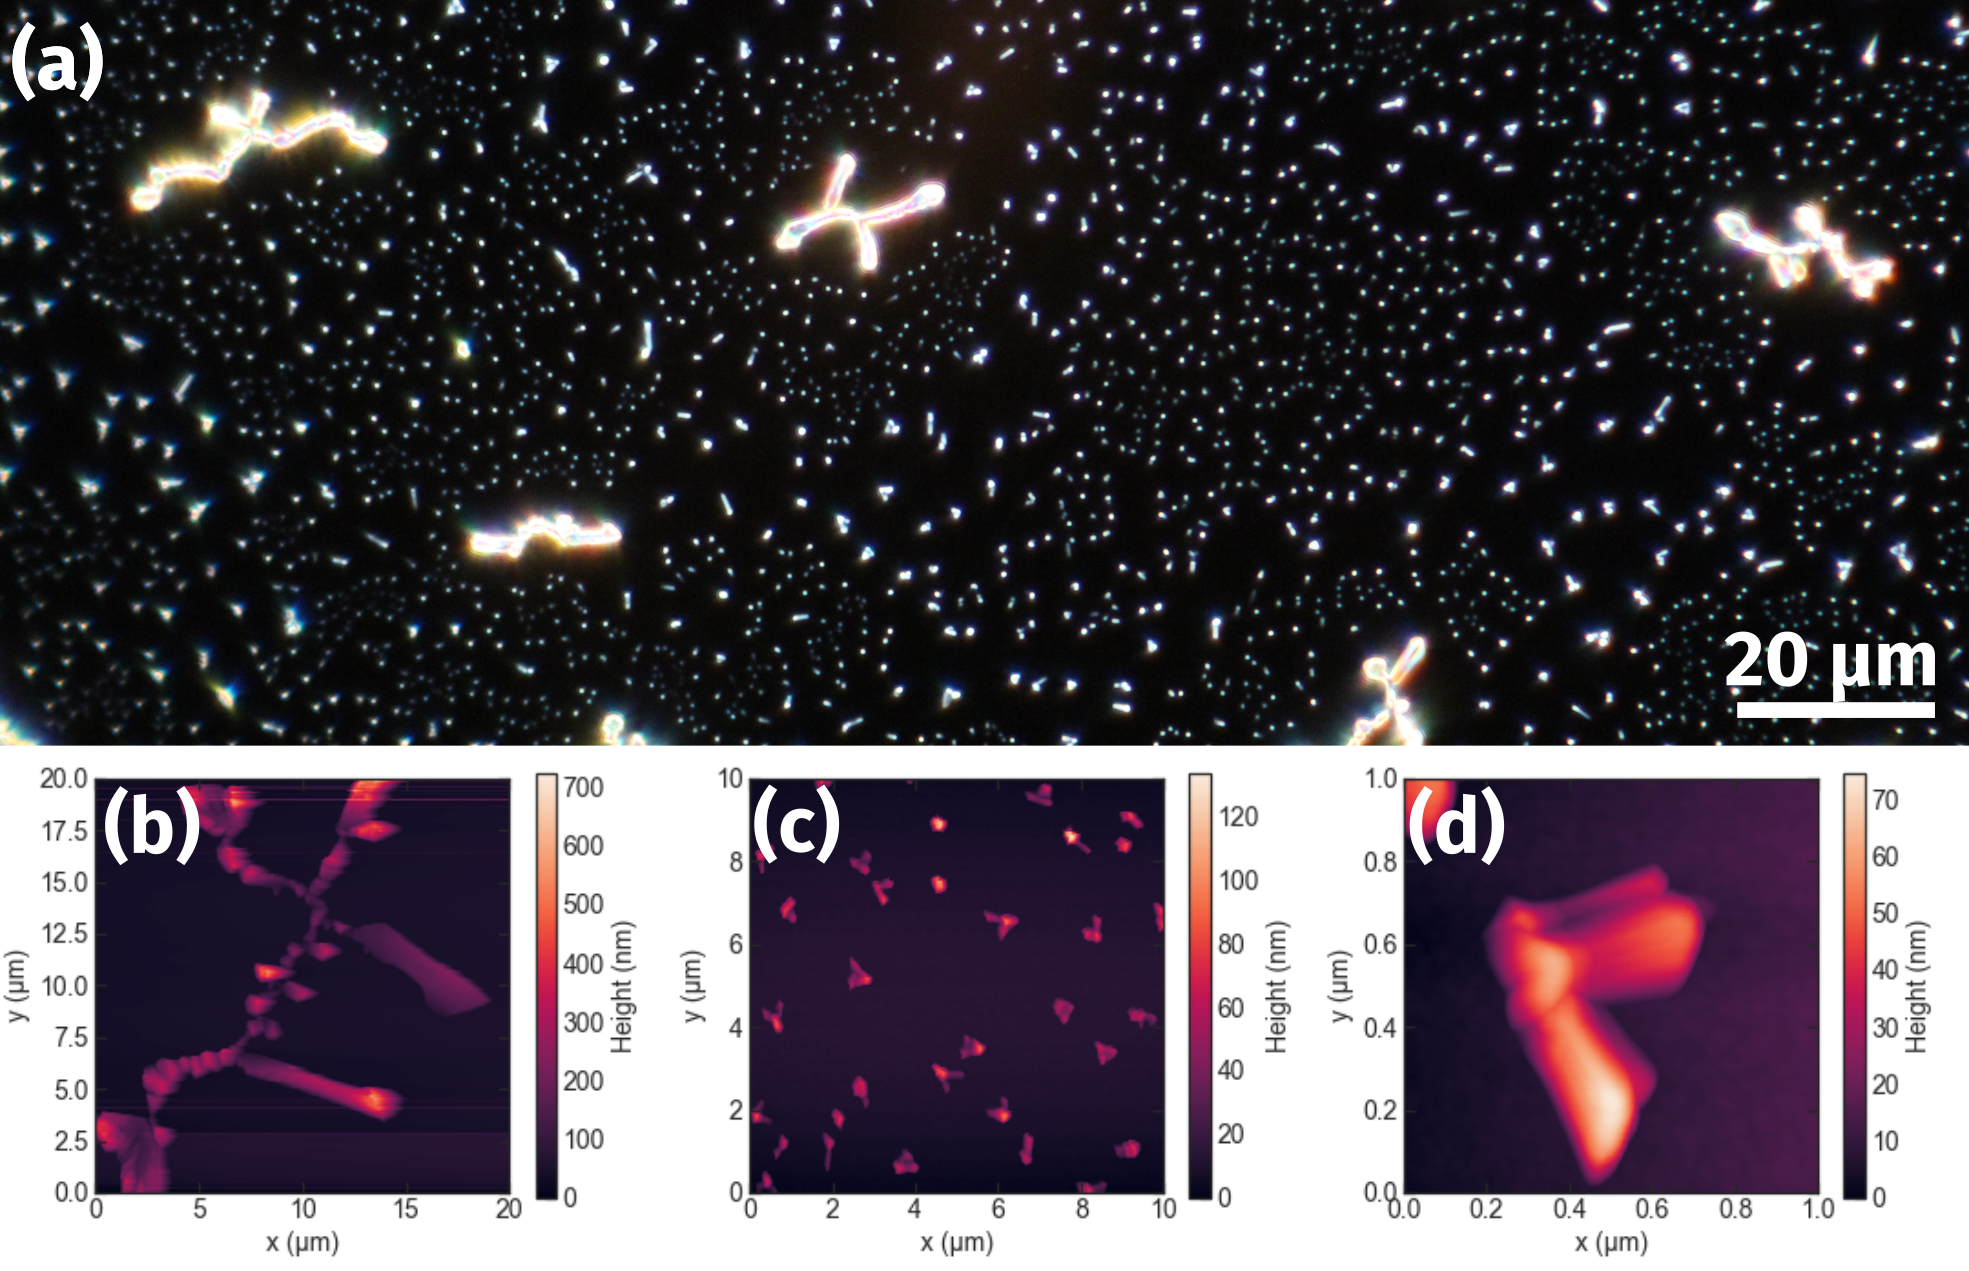
\includegraphics[]{{chapter-experimental-methods/figs-fabrication/MoreDNA.svg}.png}
	\caption{
		\textbf{DNA-like oxidation of MoRe thin films.}
		\textbf{A,} Optical image of MoRe film under and dark field after two weeks in ambient conditions.
		Scale bar \SI{25}{\micro\meter}.
		\textbf{B-D,} AFM images of several locations and types on the film:
		Small individual crystallites (B) serve as seed islands on the film surface (C), which then agglomerate into DNA-like strands (D), covering the entire film surface (A).
		MoRe film thickness \SI{100}{\nano\meter}.
	}
	\label{fig:MoreDNA}
\end{figure}

\begin{figure}
	\centering
	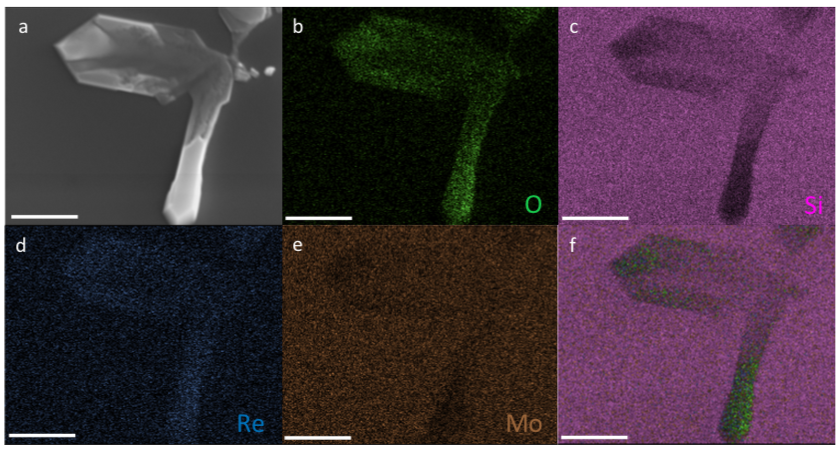
\includegraphics[width=\linewidth]{chapter-experimental-methods/figs-fabrication/pics/MoRe_EDX}
	\caption{
	\textbf{EDX spectra of MoRe crystallites on silicon substrate.}
	\textbf{a,} SEM image of a region in the MoRe layer.
	\textbf{b-e,} EDX elemental maps of O, Si, Re and Mo respectively.
	\textbf{f,} Superposition of the \textbf{b-e} elemental maps.
	All scale bars \SI{2}{\micro\meter}.
	Courtesy of Dr. Miguel Tinoco-Rivas/Conesa-Boj lab, TU Delft.
	}
	\label{fig:moreedx}
\end{figure}